\chapter{Infrastructure}\label{chap:Methods}
\section{OpenUH compiler}
OpenUH\cite{liao2007openuh}\cite{chapman2013experiences} is a branch of the open-source Open64 compiler suite which researchers in the HPCTools group at the University of Houston have developed and used to support a range of research activities in the area of programming model research. In figure~\ref{fig:openuhcompiler} shows the overall compiler infrastructure for OpenUH. Its modern and complete framework for inter- and intra-procedural state-of-art analyses and optimization is the most prominent part of Open64/OpenUH. OpenUH uses a tree-based IR called WHIRL. It comprises 5 levels, from Very High(VH) to Very Low(VL), to enable a broad range of optimizations. This design allows the compiler to perform various optimizations with proper form of IRs on different levels. 
\begin{figure}
\centering
\label{fig:openuhcompiler}
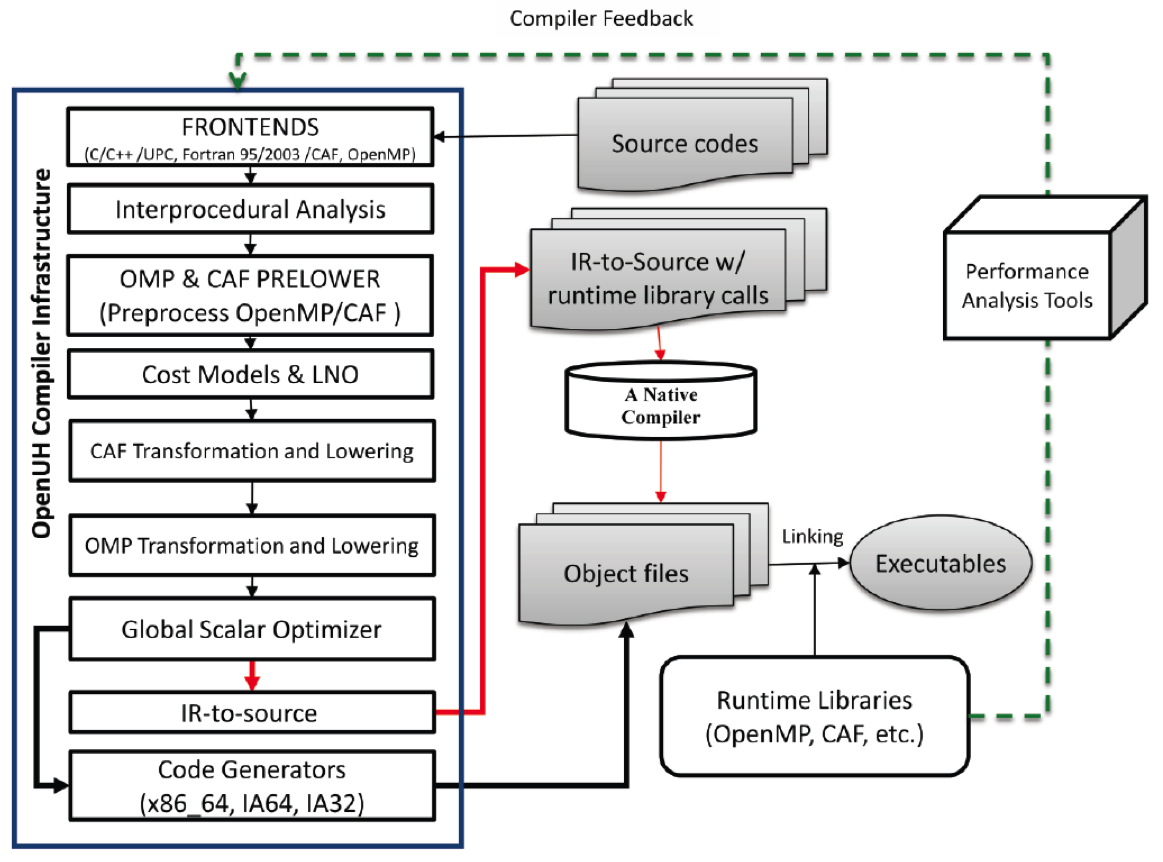
\includegraphics[scale=0.6]{figures/openuharchitecture}
\caption{OpenUH compiler infrastructure}
\end{figure}
The major functional parts of the compiler that we may concern are the C/C++ frontend and Fortran frontend, the interprocedural analyzer/optimizer(IPA/IPO) and the middle-end/back-end, which is further subdivided into the loop nest optimizer(LNO), glboal optimizer(WOPT), and code generators(CG) for 32-bit and 64-bit x86 platforms. Addtional features provided by this compiler infrastructure include the ability to emit source from an optimized intermediate representation, as well as to selectively instrument the lowered intermediate code for low-overhead performance profiling. 

The HPCTools group has undertaken a broad range of infrastructure development in OpenUH to support important topics such as language research, static analysis of parallel programs, performance analysis, task scheduling, and dynamic optimization, etc\cite{}.

OpenUH provided a solid base infrastructure for exploring implementation strategies for Coarray Fortran. The Fortran 95 frontend, which is contributed by Cray, was already capable to recognize coarrays and parsing the cosubscript syntactic extension. We took it as the start point for our implementation. The multi-level WHIRL IR, used throughout the middle-end and back-end of the compiler, provides rich support for a wide range of program abstractions. At its highest level of abstraction, VH-WHIRL, it is capable of representing Fortran array sections. This allowed us to design our back-end translator to directly map array section remote memory access into bulk communication function calls. The comprehensive optimization infrastructure available in OpenUH also provides a means for us to generate highly optimized coarray programs. OpenUH also includes its own Fortran runtime libraries, providing support for the myriad intrinsic routines defined in Fortran, memory allocation, I/O, and program termination. We chose to implement our CAF runtime outside these othter Fortran runtime libraries and reduce as much as possible its dependence on them. This would allow us to very easily port our CAF runtime to be used with different compiler.

\section{Coarray Fortran}\label{sec:coarrays}
In chapter~\ref{chap:Background} we have gone through the history of Fortran and currently active Coarray Fortran project. In this section, we will have a closer look to the parallel features that are defined and will be included in the latest Fortran language specification. 

Coarray Fortran(CAF) is a subset of the Fortran 2008 standard which adds parallel processing capabilities to the base language by adopting a SPMD model for work decomposition and \emph{coarrays} for data decomposition. In following subsections, we will go through the enssential parts of this parallel language and see some syntax examples when necessary. 

\subsection{Execution Unit}
In Coarray Fortran program, the execution unit is called \emph{image}. A Coarray Fortran program is consist a set of \emph{images} which are lanching at the beginning of program and running in parallel. The number of \emph{images} can be specified ahead of programming running but it is fixed during the execution of the program. One can set this number via compiler option, by an environement variable, or specified by options passed to a program job launcher. Each image is identified by an unique image index which start from 1 to the number of images. Two intrinsic functions \texttt{this\_image} and \texttt{num\_images} are provided for user to query about the \emph{image} identification and total number of images running during the program. Pratically, each running image is running on a separate processor but it is not necessary, and it performs computations on the data residing in its local memory. Part of images' memory are shared between images, which means other images may access to other images' memory space with a one-sided communication manner.  

\subsection{Coarrays}
These logically shared memory object are decleared and represented in CAF program as \emph{Coarrays}. Coarrays are declared with the \texttt{codimension} attribute specifier. Codimensions are analogous to array dimensions, in that they may be used to describe a multi-dimensional rectangular shape associated with a data entity. Codimensions describes the rectangular \emph{coshape} of the set of images which each contain the coarray variable in its memory. 

Coarrays may be tranfered as dummy arguments into a procedure, so long as the associated actual argument is also a coarray. Otherwise, a coarray may be decleard with either the \texttt{save} or \texttt{allocatable} attribute, for static coarrays and dynamic allocatable coarrays respectively. For non-allocatable coarrays, the \texttt{codimension} specifier should indicate the size of all codimensions except the last one for which the upper-bound must be specified as an asterisk, as shown in figure~\ref{fig:coarraydemo}. Allocatable coarrays have a \emph{deferred} coshape; the dimension bounds should specified in the \texttt{allocate} statement with the last codimension specified with an asterisk. 

Codimensions associated with a coarray provide a means to uniquely refer to a coarray located on another image, which we called \emph{image selection}. When a coarray variable is referenced with \emph{cosubscript}, similar as subscript to array selection syntax but surrounded within square brackets, the compiler will identify it as a remote memory access to the coarray at the image identified by the cosubscripts. The intrinsic functionn \texttt{image\_index} will return the image index of the image containing a specified coarray variable with a specified set of cosubscripts. Unlike the array reference, cosubscripts must uniquely refer to a single image. It cannot use subscript triplets and vector subscripts to refer more than one images at once. In Fortran, a data oject is remote accessible if it is (1) a coarray, (2) a pointer or allocatable component of a coarray, or (3) an object with the \texttt{target} attribute that is pointer associated with a pointer component of a corrary. 

\subsection{Image Control Statement}
%TODO:EDIT this part
\subsection{Teams and collectives}
As we discussed in section~\ref{sec:caf2.0}, the features in Fortran 2008 standard only provides a simple set of syntax for expressing communication and basic coordination mechanism among excuting images. The researcher in Rice University have proposed a set of new constructs and syntax to extend the CAF. Recently, the Fortran Standard committee is working on the addtional parallel features, which are described in the technical specification document\cite{caf-spec}. In this draft, they propose some language features to deal with the shortage that we have discussed in section~\ref{sec:caf2.0}. Among these features, the \emph{team} and \emph{collectives} are going to be the main topic in this thesis. We will talk about them in detail in chapter~{chap:Algorithms}.

%Researchers in Rice University have proposed their notation for subset of processes, named as \emph{team}. In the specification, the Fortran work group have proposed a similar construct, also named as \emph{team}. In the beginning of CAF program, all images are launched and included into the \emph{initial team}. During the program, all images may create a new team with \texttt{form team} statement. This statement will split current team into several \emph{sibling team}, according to the \emph{team\_id} they have specified to the statement. All the images in the current team are uniquely assigned to one of those teams. In CAF 2.0, the routine provides similar functionality is \texttt{team\_split}. Each image have a private \emph{team variable} to store the necessary information.

%Another important feature introduced into language is the collective functions. 

\subsection{Termination}
A Coarray Fortran program may terminate in one of two modes - \emph{normal terminination} or \emph{error termination}. When an image reaches to the end of a program or executes the stop statement, it will terminate properly in three steps: initiation, synchronization and completion. One image cannot terminated until all images reach the second step of normal completion. Error termination occurs when an image meets an error condition. This could occur when it encounters an error state as defined by the standard, when the program executed an \texttt{error stop} statement, or maybe it is notified that some other image is in error termination. When any image initiates error termination, the runtime should attempt to signal all images as soon as possible to shut them down and return an error status code.
\subsection{Other features}
To be noticeed that there are some other useful features or syntax on the specfication and we have supported in our compiler and runtime. I will name some of them here but I cannot go further detail about them since they are less relevent to my topic in this thesis. 

We have supported Atomic object and operations upon them. 
%TODO: EDIT: ATOMIC, EVENT
\section{GASNet}
In our CAF runtime, we chose two outstanding libraries as our communication layer, GASNet and ARMCI. In this thesis, I will only focus on the first one, GASNet, since most of my work is done and verified on top of it. GASNet\cite{bonachea2002gasnet}\cite{bonachea2002gasnetspec}, for the abbreviation of Global Address Space Networking library, is a language indenpendent runtime library developed and maintained by a research group at the University of California Berkeley and Lawrence Livermore National Laboratory. GASNet was designed to serve the UPC and Titanium, which are two famous PGAS languages with base language in C and Java. Soon it has been widely used to support a variety of PGAS implementations inluding the Co-Array Fortran and CAF 2.0 from Rice University. We also found it in Cray's UPC and CAF compiler for the CrayXT series, the Cray Chapel compiler and OpenSHMEM reference implementation, which is developed and maintained by Univeristy of Houston. 

GASNet has an API specification which defines interface for compilers or runtime system to use, which we will briefly review in this section. GASNet was designed with portability and performance in mind, and it includes implementations for many popular network APIs covering the common cluster interconnects, as well as specialized interconnects from IBM and Cray. 

A running program which uses GASNets, called the client program, consists of a set of operating system processes, or \emph{nodes}. These nodes may furthermore be grouped into supernodes, which means they are controlled by the same operating system instance. Each node may attach a \emph{segment} to its address space, which is a range of virtual addresses that are remotely access across GASNet nodes. Furthermore, the client program may execute in one of three threading modes 
\begin{itemize}
\item GASNET\_SEQ allows only one single thread on a node the make any GASNet calls
\item GASNET\_PARSYNC allos only one thread to make GASNet calls at a time
\item GASNET\_PAR provides full multi-threaded support
\end{itemize}

The GASNet API consists of a core API and an extended API. The core API provides all the facilities necessary to manage parallelism in the application, including runtime initialization and finalization, querying the environment variables in GASNet, and mutexes for multi-threaded client programs. In this thesis, the most significant part of the core API is the \emph{active message}(AM) support. This provides means to invoke registered AM handlers on a remote GASNet node. The handlers are resricted to using only a subset of the core API, and in particular they may not use the extended API for communicating with other GASNet nodes. The core API also provides support for named or unnamed split-phase barriers. 

The extended API provides support for remote memory access(RMA) operations. This includes blocking \emph{get} and \emph{put} operations, implicit-handle non-blocking \emph{get} and \emph{put}, and explicit-handle non-blocking Get and Put, and synchronization routines for waiting on completion of explicit-handle and implicit handle RMA operations. While the specificaion presently allows only contiguous remote data transfers, we can also find support for non-contiguous remote data transfer in Berkeley's implementation. 


